
\section{Results and discussion}
\label{sec:results}


For each dataset, the combination of a probabilistic degradation model and the SR model (from now on, a pipeline) was trained. 
Each pipeline has 3 main components: A generator, used to generate LR images similar to the target domain, from HR images coming from the source domain. A discriminator, used to distinguish between real LR images coming from the target domain and the generated ones. An SR model, used to super resolve the generated LR images during training.


The pipeline trained on $\mathcal{D}_{\text{SF}-\text{SF}}$, using unpaired HR-LR pairs generated by applying the baseline degradation model described in \ref{fig:3-probabilistic-degradation-model}, will be referred to as the baseline pipeline.
While the employed degradation model is stochastic, it has known parameters that are very close to bicubic downsampling + white noise. The objective is to observe how the GAN is able to imitate a known degradation model  in order to produce LR images.

The pipeline trained on $\mathcal{D}_{\text{SF}-\text{RF}}$, using unpaired synthetic HR and real LR FOREST-2 images, will be referred to as the adapted pipeline.
In this case, the degradation model is unknown and the objective of the GAN is to estimate it, generating LR images that come from the same distribution as the real FOREST-2 images.

    \subsection{Source domain}

        This subsection will analyze the results from the experiments performed on the source domain.
        The process consists of degrading the synthetic HR FOREST-2 images using the probabilistic degradation model trained through adversarial learning and then super resolving it.
        This is the equivalent of the black arrows flow described in fig. \ref{fig:3-GAN-degradation-model}. 
        As in this case the ground truth is known, the performance of the super resolution can be evaluated using metrics like PSNR and SSIM. 

        Fig. \ref{fig:5-source_domain_sample} shows the results of the baseline and the adapted pipeline, when applied to one sample from the source domain (a synthetic HR FOREST-2 image). 
        For comparison, a pipeline consisting of simple gaussian blurring + downscaling for degradation and bicubic upsampling for SR is also shown. 

        While the baseline kernel is very simple and the noise is more or less uniform across the image, the adapted kernel is more complex and the noise seems to be strongly correlated with the image intensity.

        The degraded LR images present considerable differences. While the baseline pipeline produces images very similar to gaussian blurring + downscaling, 
        the adapted pipeline produces much more blurry images with more noise, suggesting that FOREST-2 produces less resolution than what was initially expected. 
        This is also confirmed by calculating the PSNR between the LR image generated by each pipeline with the gaussian blurring + downscaling LR reference, which yields worse results for the adapted pipeline.
        
        The SR images produced by both pipelines yield better performance than bicubic interpolation, and they are very similar between them.
        This suggests that the super resolution model is able to recover the details lost during a more complex degradation processes, but there seems to be a limit to the amount of detail that can be recovered. Despite very different starting points, the final result is very similar.

        
        

        \begin{figure}[H]
            \centering

            \includegraphics[scale=0.29]{Includes/5-source-prediction-sample.pdf}
            \caption{\small{\small{Applying degradation models on an HR sample. The 2 most upper rows show the estimated kernels and noise for each pipeline (bicubic downsampling does not perform any estimation). The degraded images from each pipeline are displayed afterwards. The PSNR is calculated against the bicubic downsampling LR. The SR results are displayed in the last 2 rows. The PSNR for each SR method is calculated against the ground truth.}}
            }
            \label{fig:5-source_domain_sample}
        \end{figure}



        In Figs \ref{fig:5-lr-images-fft.pdf} the frequency domain of the LR images is analyzed.
        By inspection of the FFTs, it is observed that the adapted-LR loses more information than the baseline-LR, as the log magnitude of the FFT diminishes faster and closer to the center.
        The baseline-LR FFT is very close to the gaussian blurring + bicubic upsampling FFT, suggesting that the baseline pipeline is able to mimic this known degradation model.

        \begin{figure}[H]
            \centering
            \includegraphics[scale=0.3]{Includes/5-lr-images-fft.pdf}
            \caption{Log mangnitude of the FFT for the LR images obtained by the pipelines and the gaussian blurring + bicubic upsampling.}
            \label{fig:5-lr-images-fft.pdf}
        \end{figure}

        The radial profile of the log magnitude of the FFT for the LR images is shown in Fig. \ref{fig:5-lr-images-fft-comparison.pdf} confirms what was observed previously. When compared to bicubic downsampling + white noise,
        the adapted-LR image diminishes the high frequency components much more than the baseline-LR. This effect starts at 0.1 cycles per pixel, with a stable effect of -6dB from 0.2 to 0.5 cycles per pixel. 
        It is important to note that 0.1 cycles per pixel at a 210m GSD corresponds to a cycle frequency of 2100 $m^{-1}$, 0.2 cycles per pixel corresponds to 1050 $m^-1$ and 0.5 cycles per pixel to 420 $m^{-1}$.
        This suggests that the degradation model from the real FOREST-2 images is more complex and loses more information than the baseline degradation model.
        An analysis for the whole validation dataset will be further discussed to verify that this behaviour is consistent across different scenes and conditions.


        \begin{figure}[H]
            \centering
            \includegraphics[scale=0.45]{Includes/5-lr-images-fft-comparison.pdf}
            \caption{(a) Radial profile of the log magnitude across spatial frequency of the LR images obtained by the pipelines and the gaussian blurring + bicubic downsampling model.
                     (b) Amplification in dB of each pipeline with respect to the gaussian blurring + bicubic downsampling.}
            \label{fig:5-lr-images-fft-comparison.pdf}
        \end{figure}

        When analyzing the super resolved images versus the ground truth in the frequency domain, a very similar frequency response is observed for both pipelines.
        Moreover, the SR images are able to stay above -3dB, a common threshsold used in the literature, up until 0.2 cycles per pixel, which correspond to 350$m^{-1}$ when each pixel equals 70m.
        This suggests that the SR model in the adapted pipeline is able to recover the lost information at those frequencies due its more complex degradation model.
        Starting at 0.2 cycles per pixel, a decrease in amplification is observed for both pipelines, but more steeply for the adapted pipeline.
        This may be related to the fact that the adapted degradation model diminishes cycles at higher frequencies even more than the baseline degradation model. 
        A limit for the SR algorithm is also noted, even using a simple degradation model such as the baseline, the SR model is not able to recover higher frequencies with respect to the original, HR image.

        \begin{figure}[H]
            \centering
            \includegraphics[scale=0.5]{Includes/5-source-sr-fft-comparison.pdf}
            \caption{Frequency domain analysis of the SR images and the ground truth displayed in Fig. \ref{fig:5-source_domain_sample}.
                     In (a), the log of the magnitude of the FFT for the SR images and the ground truth is shown,
                     while in (b), the amplification of each SR image with respect to the ground truth is shown.}
            \label{fig:5-source-sr-fft-comparison}
        \end{figure}

        \subsubsection{Probabilistic degradation models comparison}

        In order to better understand the stochastic nature of the generator, a kernel was extracted 2000 times from it using different realizations of the random variable $z_k$.
        The mean and standard deviation of the sampled kernels was then computed.
        It is important to note that the experiment configuration assumes that the kernel does not depend on the pixel content or position, resulting in one kernel per image.
        The results are shown in Fig. \ref{fig:5-source-kernel-mean-std}. 
        In order to make the standard deviation of each pixel comparable, its value is normalized by the mean of the corresponding pixel. 
        This allows to express the standard deviation as a percentage of the corresponding pixel  mean value.
        
        While the baseline and the adapted kernel have the maximum mean and std in the same pixel, the adapted one denotes a bigger surface.  
        The baseline kernel is composed of a few pixels very close to each other.
        Additionally, the maximum mean in the baseline model is close to 0.7, while the value for the adapted one is close to 0.1.
        This suggests that the adapted kernel is more complex and spread out, while the baseline kernel is simpler and more concentrated.
        As a result, the adapted kernel produces more blurry images.
        
        The figure also displays the benefits of the probabilistic degradation model.
        Using only one HR image, the generator is able to produce a wide variety of LR pairs. Allowing the training of SR models  to generalize better.

        \begin{figure}[H]
            \centering
            \includegraphics[width=\textwidth]{Includes/5-source-kernel-mean-std.pdf}
            \caption{Mean and standard deviation of the estimated kernels for the baseline and adapted degradation model, using 2000 realizations of $z_k$.
                     The standard deviation of each pixel is normalized by the corresponding mean value. Kernel pixels with mean lower than $10^{-4}$ are considered with 0 std for clarity in the plot.}
            \label{fig:5-source-kernel-mean-std}
        \end{figure}

        In the case of the noise, the experiment setup assumes that it depends on the pixel content and position.
        For that reason, two different characterizations were done. 
        First, The stochastic component of the noise will be assessed by computing the SNR between the clean image $I^{\text{LR}}_{\text{clean}}$ product of the convolution between $I_{\text{HR}}$ and the kernel, and the output of the noise module, using 2000 different realizations of $z_n$.
        Similar what happens on the kernel, several noise levels can be added to the same image, in order to enrich the dataset even more. It can also be noted that for this particular image, the SNR of the baseline model is higher.

        
        \begin{figure}[H]
            \centering
            \includegraphics[width=\textwidth]{Includes/5-source-noise-1-sample.pdf}
            \caption{Distribution of SNR values using $I^{\text{LR}}_{\text{clean}}$, product of the convolution of the kernel and $I^{\text{HR}}_{\text{clean}}$, and the noise module output for both pipelines.
                     The output noise is generated 2000 times, using different realizations of the random variable $z_n$ for each iteration and the same input image.
                    }
            \label{fig:5-source-noise-1-sample}
        \end{figure}
        

        Second, and to further analyze the differences in SNRs between the degradation models, the ratio will be computed whole validation dataset.
        An estimated density function of the SNR for pipeline is shown in Fig. \ref{fig:5-source-noise-SNR}.
        The SNR is in general bigger when using the baseline model compared to the adapted one.
        This implies that in the output of the adapted model generator, the noise tends to have more power. 

        \begin{figure}[H]
            \centering
            \includegraphics[width=\textwidth]{Includes/5-source-noise-SNR.pdf}
            \caption{Comparison of the SNR expressed in dB of the low resolution images generated by the baseline and adapted degradation model.}
            \label{fig:5-source-noise-SNR}
        \end{figure}


        A similar procedure is performed but calculating the pearson correlation coefficient between the input image $I^{\text{LR}}_{\text{clean}}$ and the output of the noise module. The adapted degradation model produces noise highly correlated with the input.


        \begin{figure}[H]
            \centering
            \includegraphics[width=\textwidth]{Includes/5-source-noise-correlation.pdf}
            \caption{Comparison of the Pearson correlation coefficient between $I^{\text{LR}}_{\text{clean}}$ and the output of the noise module for the baseline and adapted degradation model.}
            \label{fig:5-source-noise-correlation}
        \end{figure}

        

        The observed effects support what is observed in the Fig. \ref{fig:5-source-domain-comparison}. 
        The adapted pipeline produces broader kernels and noise with more energy that is highly correlated with the image content, compared to the baseline pipeline.
        This leads to more blurry and more noisy generated LR images. 
        The kernel imposes a low pass filter for the frequency components in the image, and the noise degrades the amount of recoverable signal from it.
        Both components will create a more difficult scenario for the SR model. 

        \subsubsection{Low resolution images comparison} \label{subsec:results-lr-comparison}

        A quantitative analysis of the LR images obtained by the generator of each pipeline is performed. 
        Fig. \ref{fig:5-source-domain-lr-performance-scatterplot} shows 3 supervised performance metrics obtained by comparing the LR images obtained by the pipelines with the gaussian blurring + bicubic downsampling degradation.
        In this case, a consistent higher PSNR and SSIM means that the baseline-LR image is closer to the gaussian blurring + bicubic downsampling LR image than the one generated by the adapted pipeline. 
        A lower LPIPS means that even using perceptual metrics, the baseline-LR image is also closer.
        This is consistent with the results shown in Fig. \ref{fig:5-source_domain_sample}, where the adapted LR image is more blurry and noisy, suggesting that the unknown degradation is far from the baseline degradation model.
        
        \begin{figure}[H]
            \centering
            \includegraphics[width=\textwidth]{Includes/5-source-domain-lr-performance-scatterplot.pdf}
            \caption{Performance metrics between the LR images obtained by the pipelines vs the gaussian blurring + bicubic downsampling degradation.
                     On the left, the PSNR is displayed. On the middle and the right, SSIM and LPIPS are represented respectively.}
            \label{fig:5-source-domain-lr-performance-scatterplot}
        \end{figure}




        An alternative way to evaluate the differences in the degradations is by analyzing the frequency domain of the LR images.
        An analysis of the whole validation dataset is performed by calculating the FFT of each LR image and comparing them with the gaussian blurring + bicubic downsmapling degradation model.
        The results are displayed  in Fig. \ref{fig:5-lr-images-fft-comparison}. 
        In (a) the log magnitude of the FFT across different spatial frequency values for the degraded images is shown. 
        The spatial frequency is obtained from the radial distance to the center of the FFT, as shown in \ref{subsubsec:frequency_domain_analysis}.
        In (b), the amplification of each generated LR image with respect to a simple gaussian blurring + downscaling is shown. 
        The results for the whole dataset show that the LR images generated by the adapted pipeline yield a reduction in all frequency components consistently across all samples, with a ± 1 standard deviation interval between -4 and -8 dB from between 0.25 and 0.5 cycles per 210m pixel.

        \begin{figure}[H]
            \centering
            \includegraphics[scale=0.5]{Includes/5-source-lr-amplification-statistics.pdf}
            \caption{Frequency domain analysis of the LR images obtained by applying different degradation models on the HR sample displayed in Fig. \ref{fig:5-source_domain_sample}.
                     In (a), the log of the magnitude of the FFT for the LR images is shown,
                     while in (b), the amplification with respect to a  simple gaussian blurring + downscaling is shown.
                     The painted area represents the ±1 standard deviation of the radial profiles and the amplification. }
            \label{fig:5-lr-images-fft-comparison}
        \end{figure}




        \subsubsection{Effects of the degradation model in super resolution performance}

        Another subject of interest is how the degradation model affects the performance of the super resolution process.
        Fig. \ref{fig:5-source-domain-comparison} shows the performance obtained by super resolving the output of each pipeline generator for the whole validation dataset.
        In (a)  the corresponding SR model of each pipeline is used to obtain the super resolved images. 
        The performance, both in PSNR and SSIM, are very similar. The LPIPS shows a consistent behavior too.
        In (b), the SR model is discarded and a simple bicubic upsampling is used to super resolve the degraded images of each pipeline. 
        In this case, using the baseline LR version as input consistently yields better results than the adapted LR version, in all metrics.
        This suggests that the learned degradation model from FOREST-2 images loses more information than the baseline, resulting in a lower effective ground sampling distance than what was is specified in FOREST-2 fact sheet.
        Consistent with what was found in Figs. \ref{fig:5-source_domain_sample} and \ref{fig:5-source-sr-fft-comparison}, the SR model is able to recover most of the information, as the performance when employing the SR models is very similar. 
        
        \begin{figure}[H]
            \centering
            \includegraphics[width=\textwidth]{Includes/5-source-domain-comparison.png}
            \caption{Performance obtained by super resolving the degraded images coming out of the generator. 
                     In (a), the corresponding SR model of each pipeline is used. 
                     In (b), a simple bicubic upsampling is used to super resolve the degraded images instead of the SR model. The Pearson correlation coefficient is represented by $\rho$. }
            \label{fig:5-source-domain-comparison}
        \end{figure}

        Fig \ref{fig:5-source-domain-comparison} proves the relevance of the domain gap in super resolution, the SR model is able to estimate the inverse of the degradation function, if given the correct data.
        The problem relies on that in most experiments, the wrong degradation is shown to the model, forcing it to learn the inverse of an incorrect function.  
        This plays an essential role when applying super resolution models in real data, where the degradation model may not be known. 

    \subsection{Target domain}

        This subsection will show the results from the experiments performed on the target domain, which is the equivalent of the red arrows flow described in fig. \ref{fig:3-GAN-degradation-model}.
        In this case, the GAN trained for the degradation model is discarded and only the SR model is used with real images FOREST-2 as input.
        
        Due to the unpaired nature of the dataset, the performance of the SR model can not be evaluated using metrics like PSNR and SSIM. 
        Other alternatives will be presented, and a qualitative analysis will be performed. 
        % Additionally, a quantitative analysis will be discussed using a very small sample of paired data obtained by synchronizing the overpass of FOREST-2 with the route of ECOSTRESS.


        In Fig. \ref{fig:5-target_prediction_sample}, the super resolution models were used with a 264x264 pixels crop of a real FOREST-2 image as an input.
        The results show that the baseline model has very similar results to bicubic upsampling.
        On the other side, the adapted model, trained using real FOREST images as the target domain produces sharper images without clearly increasing the overall noise.
        
        


        \begin{figure}[H]
            \centering
            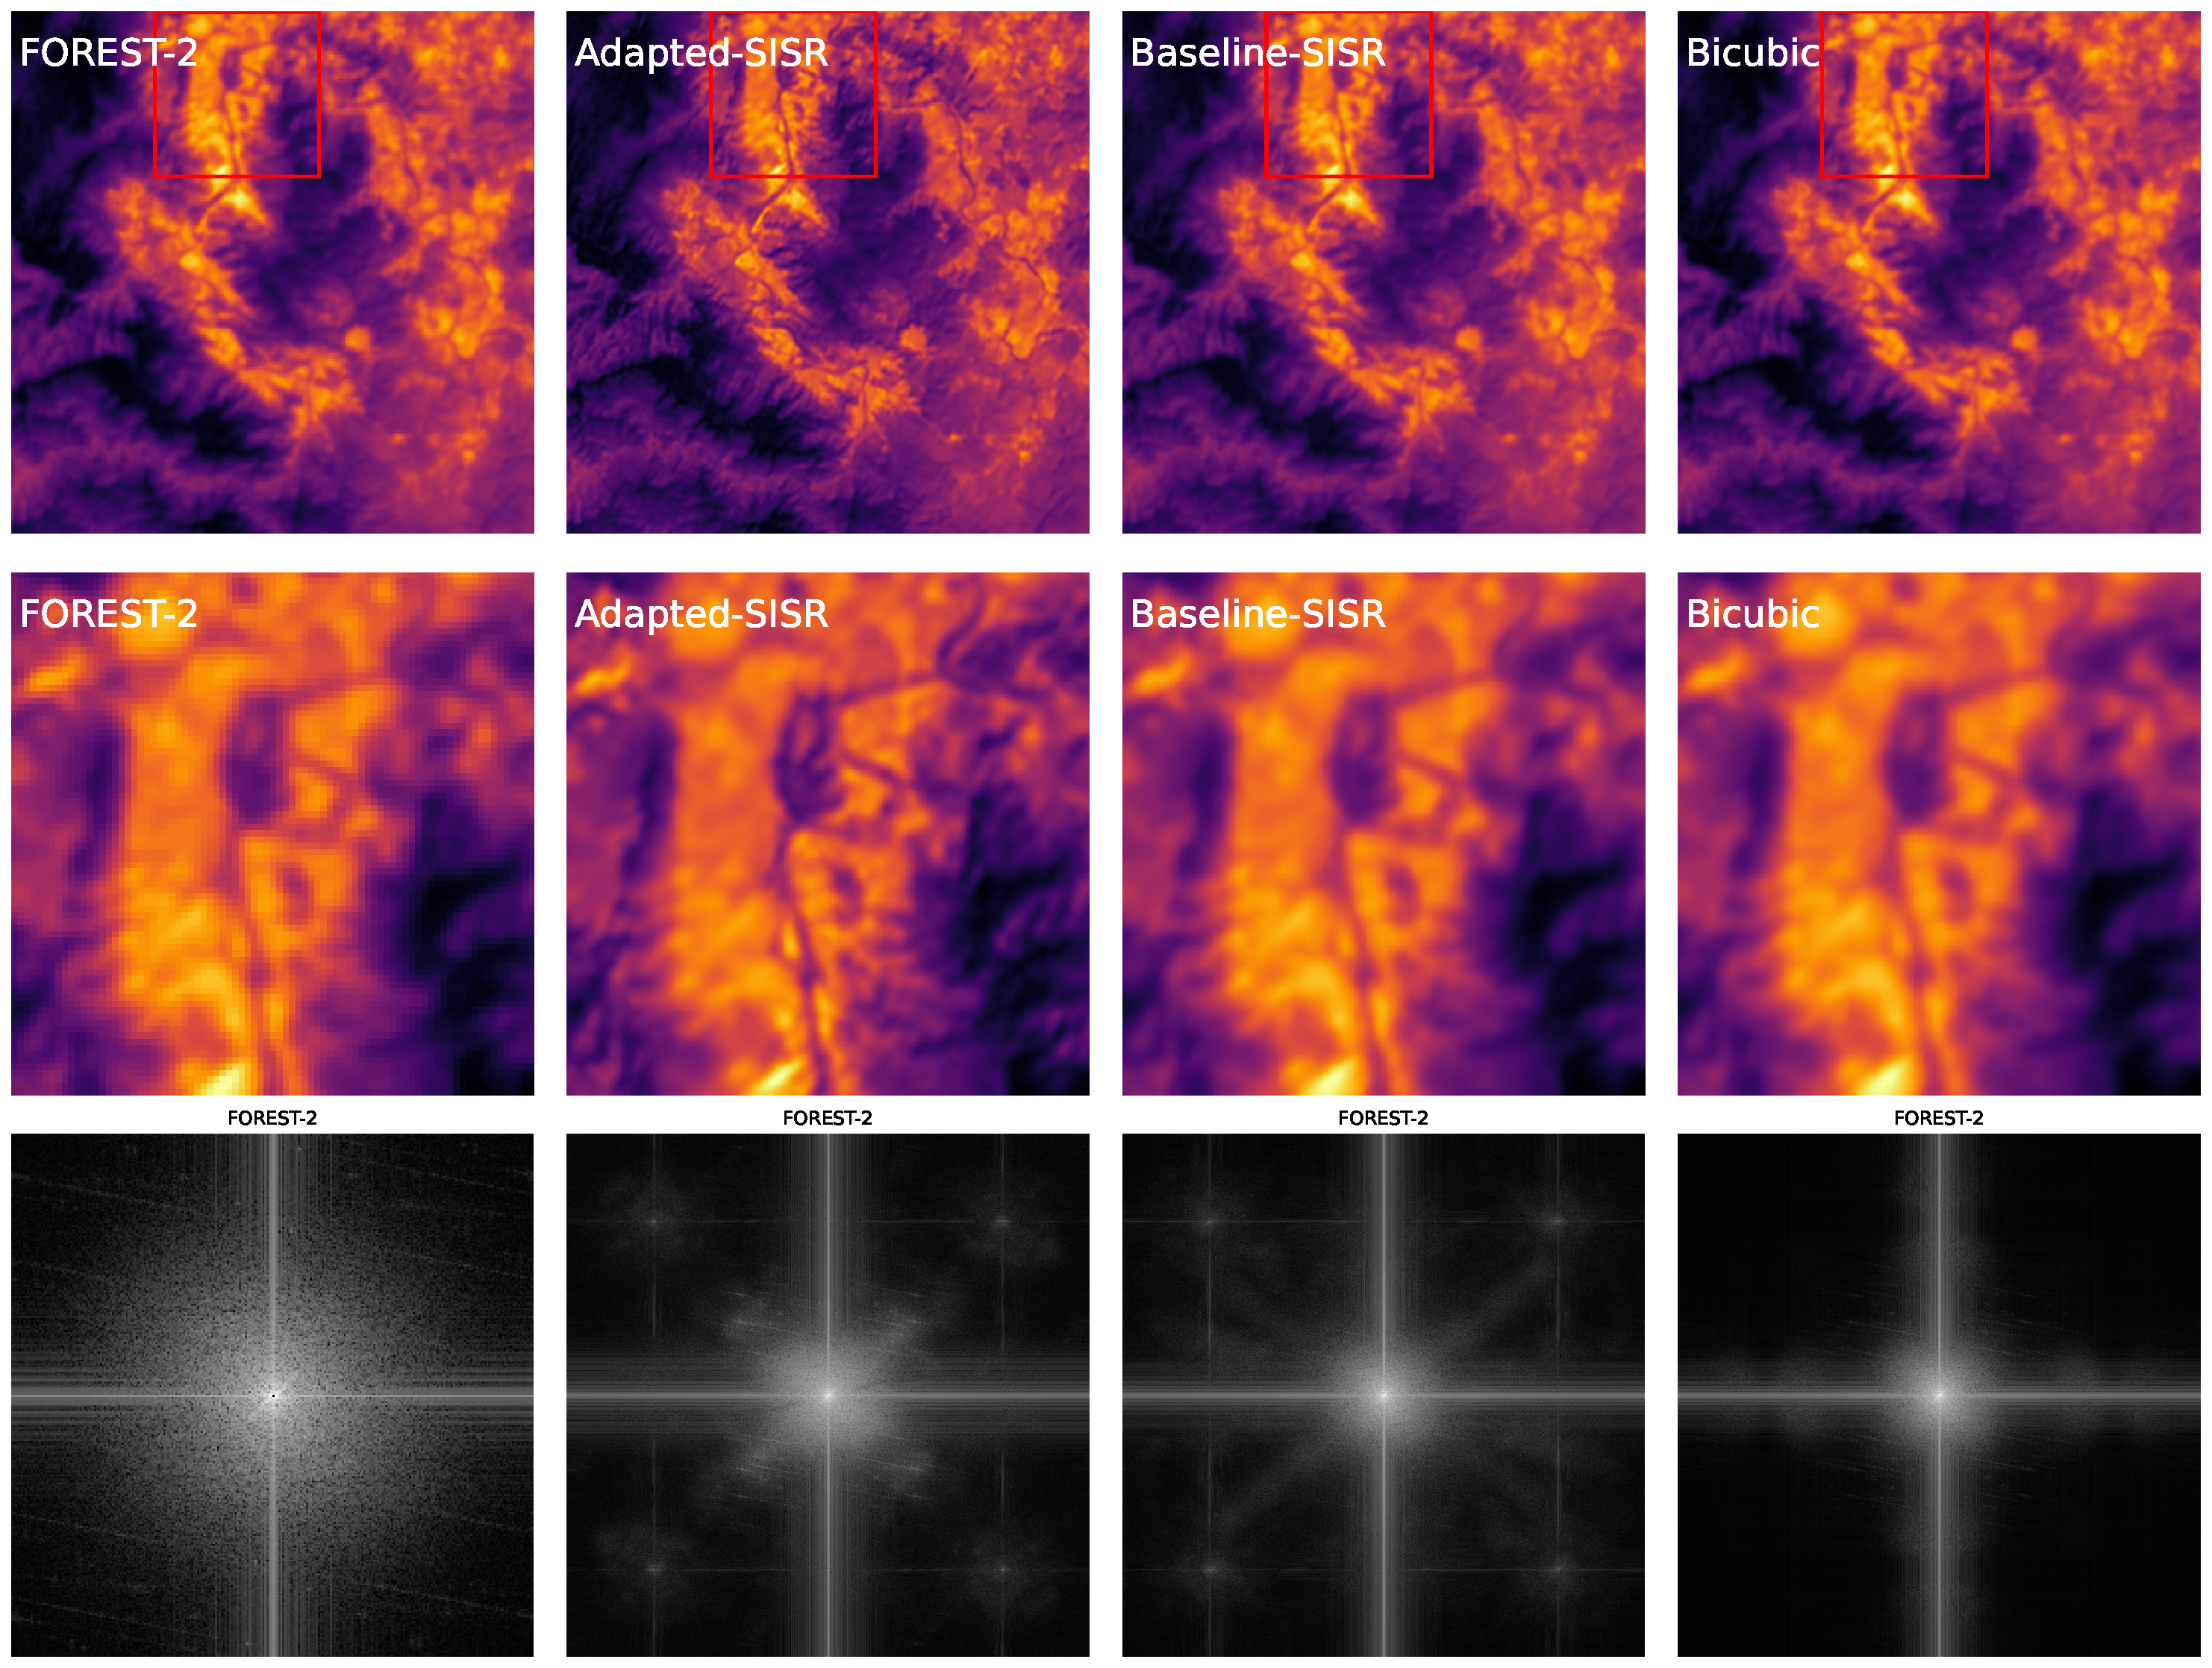
\includegraphics[scale=0.28]{Includes/5-target_prediction_sample.pdf}
            \caption{Super Resolved Forest-2 Scene using different SR models.
                     In the upper row, the image is displayed. A detailed zoom is displayed below. The original image is displayed in the left, while the super resolved images are displayed afterwards.
                    }
            \label{fig:5-target_prediction_sample}
        \end{figure}

        Fig. \ref{fig:5-target-amplification-statistics} shows a more detailed analysis of the frequency domain of the SR images obtained for the whole real FOREST-2 validation dataset.
        The effects of super resolution are clear, frequency components of interest are amplified in comparison to bicubic upsampling, without over-amplifying higher frequencies usually related to noise.  In (a),the log magnitude of the FFT for the SR images is displayed, adding a shade that represents the interval of ±1 standard deviations. 
        Up until 0.3 cycles per pixel, the adapted model has a higher log magnitude than the baseline SR model or bicubic upsampling, also staying slightly higher in high frequency components.
        As higher frequencies are related to noise and artifacts, this suggests that the adapted model is able to recover more details than the baseline model, while minimizing undesired components.
        The amplification plot of the SR models against bicubic upsampling shows the same behaviour in a more clear way. 
        The adapted amplification increases from the start of the plot and peaks between 0.08 and 0.25 cycles per pixel in a range of between 6 and 8 dB, on average, while the baseline model amplification lies between 0 and 2 dB.
        Such amplification, at a pixel size of 70m, corresponds to cycle frequencies between  300 $\frac{1}{m}$ and 875 $\frac{1}{m}$, which is consistent with the lost frequency components observed in \ref{fig:5-lr-images-fft-comparison}.
        
        On the other side, while the amplification is very similar in frequencies related to noise, the adapted model seems to step up a little bit compared to the baseline.  
        This suggests that the adapted model is able to recover details from real FOREST-2 images, amplifying frequencies of interest, at the cost of a small increase in the overall noise of the image.

        \begin{figure}[H]
            \centering
            \includegraphics[scale=0.5]{Includes/5-target-amplification-statistics.pdf}
            \caption{Frequency domain analysis of the SR images obtained by applying different SR models to the real FOREST-2 validation dataset.
            In (a), the log of the magnitude of the FFT for the SR images is shown,
            while in (b) the amplification with respect to a  simple bicubic upsampling is displayed.}
            \label{fig:5-target-amplification-statistics}
        \end{figure}


        In Fig. \ref{fig:6-target-gradient-analysis-image}, an example of the gradient analysis of the SR images is shown. 
        Compared to the baseline SISR model, the adapted model shows higher gradient magnitudes, suggesting that the adapted model is able to recover more details than the baseline model. 
        However, in the darker sections of the gradient magnitude, some small background noise can be observed, consistent with slightly increased amplification in the higher components of the frequency domain analysis from Fig. \ref{fig:5-target-amplification-statistics}.

        \begin{figure}[H]
            \centering
            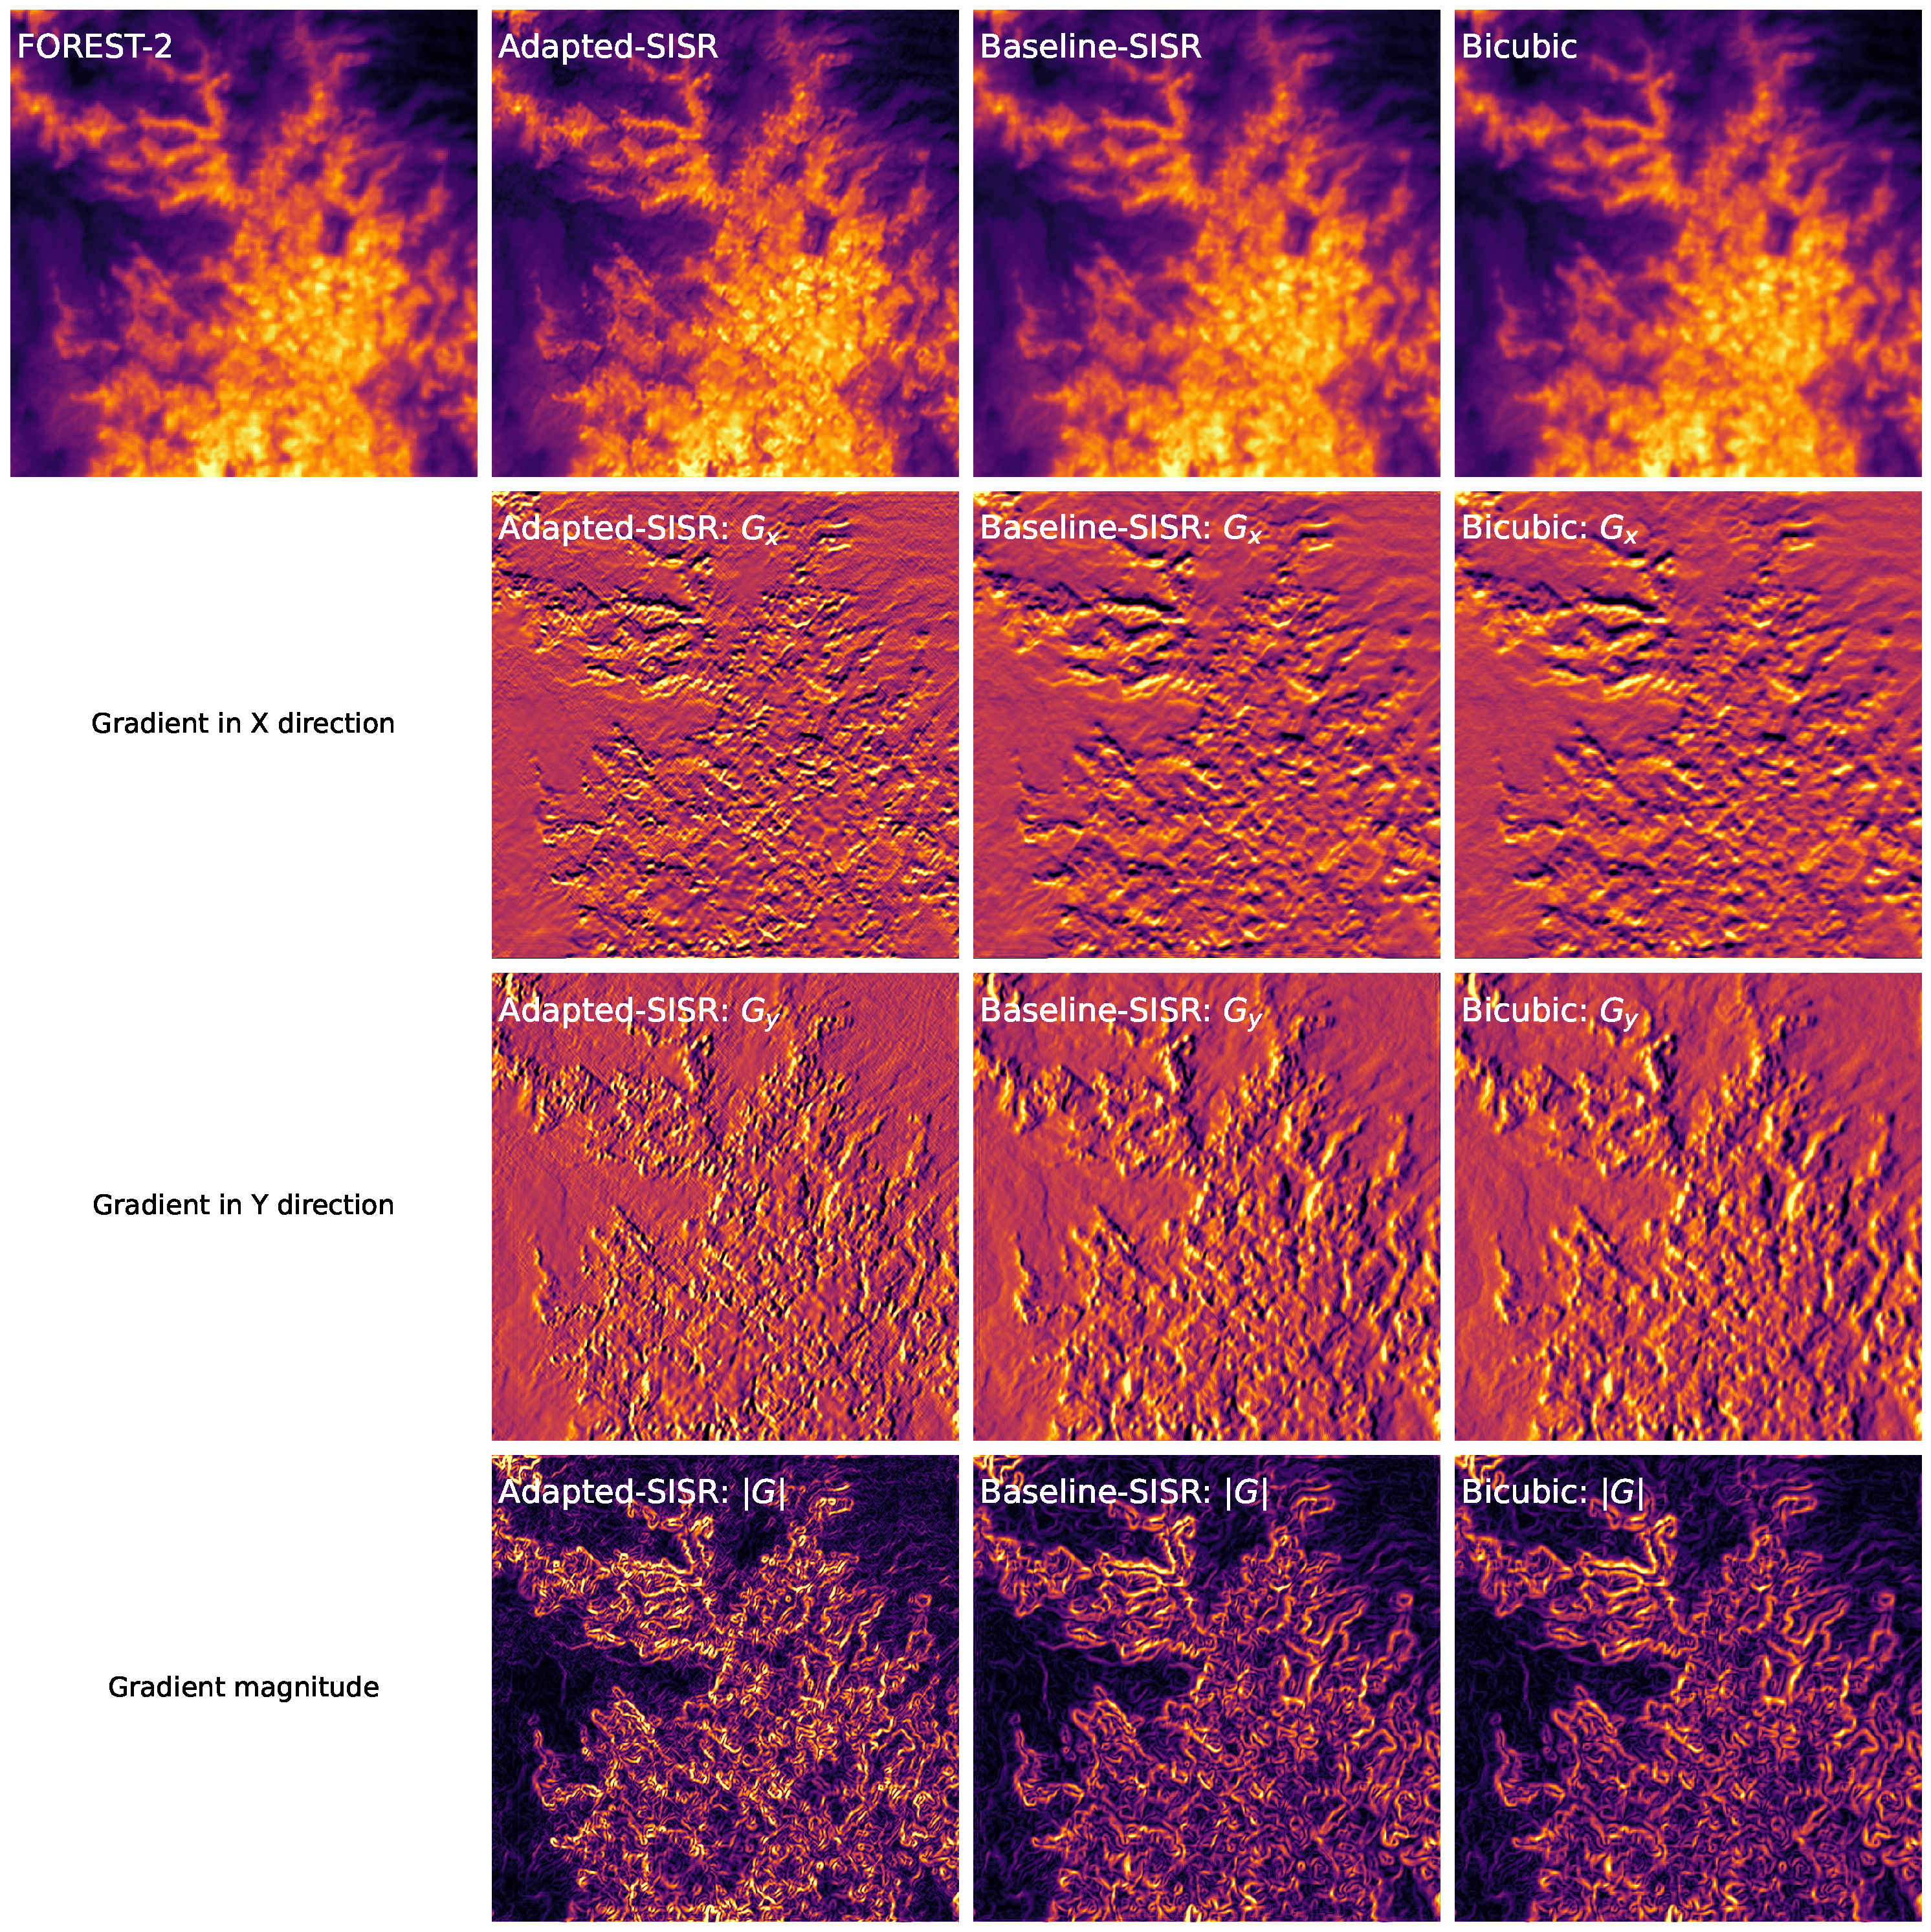
\includegraphics[scale=0.28]{Includes/6-target-gradient-analysis-image.pdf}
            \caption{Gradient analysis of the super resolved images using different SR models for scenes coming from the real FOREST-2 validation dataset.
                     In the upper row, the image is displayed. The gradients in the x and y direction ($G_x$ and $G_y$ respectiely) are displayed below.
                     the gradient magnitude $|G|$ is displayed in the bottom row.}
            \label{fig:6-target-gradient-analysis-image}
        \end{figure}

        Fig \ref{fig:5-gradient-histogram-validation-dataset} shows the estimated distribution function of the log gradient magnitudes of the whole validation dataset.
        Both the adapted and the baseline model show a decrease in the number of pixels with low gradient magnitudes compared to bicubic upsampling, suggesting that both models are able to recover more details.
        However, the adapted SR tends to have a higher high gradient magnitude pixels, implying that the adapted model is able to produce sharper edges than the baseline model.
        This is consistent with the observed results and the frequency domain analysis.
        % However, it is important to note that the gradient magnitude is not a good measure of the performance of the SR model, as it does not take into account the noise and artifacts that may be present in the image.
        % It represents only a complementary way to understand the effects of the SR model.

        \begin{figure}[H]
            \centering
            \includegraphics[scale=0.4]{Includes/5-gradient-histogram-validation-dataset.pdf}
            \caption{Density estimation of the gradient magnitude $|G|$ for the super resolved real FOREST-2 images from the validation dataset. The magnitudes of the Synthetic HR FOREST-2 images are also computed for comparison.}
            \label{fig:5-gradient-histogram-validation-dataset}
        \end{figure}

        In Fig. \ref{fig:5-correlation-histogram-validation-dataset}, the estimated density of the correlation coefficient between the pixels of an image and their neighbors is displayed for the whole validation dataset. 
        
        As expected for an image, the correlation is extremely high and the density is highly concentrated. The baseline and bicubic upsampling models have a very similar distribution, with the baseline SR being slighly skewed to the left.
        The adapted model has a broader distribution, less dense when closer to 1, implying that the pixels tend to be less correlated with their neighborhood. 
        
        \begin{figure}[H]
            \centering
            \includegraphics[scale=0.35]{Includes/5-correlation-histogram-validation-dataset.pdf}
            \caption{Density estimation of the correlation coefficient between the pixels and their neighborhoods, for the super resolved real FOREST-2 images from the validation dataset. The coefficients of the synthetic HR FOREST-2 images are also computed for comparison.}
            \label{fig:5-correlation-histogram-validation-dataset}
        \end{figure}

    \subsection{Sensibility to domain gap}

         % Another example would be images taken from FOREST-2 in several years may not have the same distribution as current images, as the instruments may have degraded over time.

        % To simulate this situation, the model trained using real FOREST-2 images was employed to super-resolve synthetic FOREST images degraded using the baseline degradation model. The results, shown in Figs. \ref{fig:5-target-prediction-with-domain-gap} and \ref{fig:5-target-prediction-with-domain-gap-fft}, indicate the performance of the adapted model is catastrophic, producing several artifacts and yielding a PSNR difference of approximately 10dB, which represents a tenfold difference in terms of Mean Squared Error (MSE). This highlights the critical need for adaptable SR models that can effectively handle diverse and evolving real-world scenarios.


        The combination of the probabilistic degradation model and the SR model were proven helpful to bridge the domain gap and improve the resolution of real FOREST-2 images.
        However, it is important to understand what happens when an arbitrary LR input that is not aligned with the target domain used in training is used.
        While the common scenario is that the real degradation model is more complex than the one assumed in the dataset generation, the opposite can also occur.
        As seen in \ref{subsec:results-lr-comparison}, assuming a more complex degradation model in the dataset could lead to LR inputs with more attenuation in critical frequency components, resulting in an SR model that "over-amplifies" to generate an HR output, leading to noisy images with undesired artifacts.
        In this particular experiments, HR-LR pairs generated using the baseline degradation model exemplify an overly optimistic degradation scenario and will be used on the SR models of each pipeline.
        As in this experiment the ground truth is known, the performance of the SR model can be evaluated using metrics like PSNR and SSIM. Additionally, a frequency domain analysis with respect to the ground truth can be done.
        
        The results are shown in Figs. \ref{fig:5-target-prediction-with-domain-gap} and \ref{fig:5-target-prediction-with-domain-gap-fft}.
        The performance of the adapted model on LR images coming from the baseline degradation model is catastrophic, producing several artifacts and yielding a PSNR difference of approximately 10dB, which represent a 10x difference in terms of MSE.

        \begin{figure}[H]
            \centering
            \includegraphics[scale=0.28]{Includes/5-target_prediction_sample-with-domain-gap.pdf}
            \caption{Effects of using a model trained  on a different domain than at inference time. 
                     When using an Synthetic FOREST image degraded with the baseline degradation model as an input, the model trained using real FOREST-2 data as the target domain generates several artifacts and underperforms severely in terms of PSNR. }
            \label{fig:5-target-prediction-with-domain-gap}
        \end{figure}

        The frequency domain analysis of the ground truth and the super resolved images are shown in Fig. \ref{fig:5-target-prediction-with-domain-gap-fft}.  
        The adapted model amplifies frequencies with respect to the ground truth, something that should not happen in any SR task. 
        This suggests that while the adapted model may highlight edges and details, it also severely amplifies the noise and artifacts, resulting in a worse performance in terms of PSNR.
        

        \begin{figure}[H]
            \centering
            \includegraphics[scale=0.4]{Includes/5-target-prediction-with-domain-gap-fft.pdf}
            \caption{Effects of using a model trained with on different domain than at inference time. 
                     (a) shows the log magnitude of the radial average of the FFT for the SR images using different algorithms.
                     (b) shows the amplification with respect to bicubic interpolation.
                     }
            \label{fig:5-target-prediction-with-domain-gap-fft}
        \end{figure}

        Fig \ref{fig:5-target-amplification-statistics-with-domain-gap} shows the results of the frequency domain analysis for the whole validation dataset. The results seem to be consistent in the range observed in Fig. \ref{fig:5-target-prediction-with-domain-gap-fft}. Having frequency amplification with respect to the ground truth is a display of the inability of the adapted SR model to reconstruct the ground truth image properly.
        
        The adapted model was trained on generated LR images that try to mimic the real FOREST-2 images, which have a more complex degradation model. This results in an SR model that tries to reconstruct the ground truth from a "blurrier" starting point, learning to amplify some frequencies much more than what is needed when the LR images come from the baseline degradation model.


        \begin{figure}[H]
            \centering
            \includegraphics[scale=0.4]{Includes/5-target-amplification-statistics-with-domain-gap.pdf}
            \caption{Effects of using a model trained with on different domain than at inference time, statistics over the whole validation dataset. 
                     (a) shows the log magnitude of the radial average of the FFT for the SR images using different algorithms.
                     (b) shows the amplification with respect to bicubic interpolation.
                     Painted areas represent ±1 standard deviations.
                     }
            \label{fig:5-target-amplification-statistics-with-domain-gap}
        \end{figure}

        The performance results in terms of different metrics are shown in Fig. \ref{fig:5-target-prediction-with-domain-gap-dataset}. 
        In the conditions described above, the adapted super resolution model underperforms severly in every considered metric.


        \begin{figure}[H]
            \centering
            \includegraphics[scale=0.38]{Includes/5-target-prediction-with-domain-gap-dataset.pdf}
            \caption{Performance obtained by super resolving the degraded synthetic FOREST images using different super resolution models. The Pearson correlation coefficient is represented by $\rho$.}
            \label{fig:5-target-prediction-with-domain-gap-dataset}
        \end{figure}
        
        
    This demonstrates that while this approach is very good to bridge a domain gap, it is not robust at all to domain shifts. 
    This limitation is in sync with what is found in the literature seen in \ref{subsubsec:implicit-modelling}. Implicit modelling for blind super resolution using GANs are not able to generalize to arbitrary domains not seen in the target domain.

    \subsection{Domain gap assessment using non-referenced image quality assessment}

    As in the target domain the ground truth is not known due to the lack of a paired dataset, the performance of the SR model can not be evaluated using metrics like PSNR and SSIM.
    Non-referenced image quality assessment (NR-IQA) metrics can help to understand the relative performance of the SR models when arbitrary LR images are used as an input.
    
    The analysis was performed by taking the adapted and baseline SR models and using them to super resolve LR images coming from the baseline degradation and real LR forest-2 images as an input.
    Then, the NIQE and BRISQUE scores are calculated.
    
    The results are shown in Fig. \ref{fig:5-target-iqa-results}.
    For both metrics, a large gap is observed between the adapted model and the rest when the input is real FOREST-2 data.
    This behaviour does not replicates when the input LR images are generated using the baseline degradation. Moreover, for the adapted model, both metrics tend to get worse when the input images are not real FOREST-2 images. The contrary happens for the rest of the models.

    \begin{figure}[H]
        \centering
        \includegraphics[scale=0.25]{Includes/5-target-iqa-results.pdf}
        \caption{Image quality assessment metrics for the different SR models using different datasets as input. }
        \label{fig:5-target-iqa-results}
    \end{figure}

    
    This suggests that the SR model is able to produce more natural images only when the input images come from the same distribution as the target domain used in training. However, it is important to note that: 

    


    \begin{enumerate}
        \item NIQE and BRISQUE are calculated using a pre-trained model. The images used for the pre-training are not remote sensing images, and therefore, the results may not be representative. This could be circumvented by training a NIQE/BRISQUE model trained with a more adequate dataset for the task.
        \item NIQE and BRISQUE are a measure of image quality and naturalness, not physical consistency or reconstruction fidelity.
    \end{enumerate}
        
\newpage
    